\documentclass{article}

% if you need to pass options to natbib, use, e.g.:
% \PassOptionsToPackage{numbers, compress}{natbib}
% before loading nips_2016
%
% to avoid loading the natbib package, add option nonatbib:
% \usepackage[nonatbib]{nips_2016}

\usepackage[final]{nips_2016}

% to compile a camera-ready version, add the [final] option, e.g.:
% \usepackage[final]{nips_2016}

\usepackage[utf8]{inputenc} % allow utf-8 input
\usepackage[T1]{fontenc}    % use 8-bit T1 fonts
\usepackage{hyperref}       % hyperlinks
\usepackage{url}            % simple URL typesetting
\usepackage{booktabs}       % professional-quality tables
\usepackage{amsfonts}       % blackboard math symbols
\usepackage{nicefrac}       % compact symbols for 1/2, etc.
\usepackage{microtype}      % microtypography
\usepackage{graphicx}

\title{Report for the Deep Learning Course Assignment 3}

% The \author macro works with any number of authors. There are two
% commands used to separate the names and addresses of multiple
% authors: \And and \AND.
%
% Using \And between authors leaves it to LaTeX to determine where to
% break the lines. Using \AND forces a line break at that point. So,
% if LaTeX puts 3 of 4 authors names on the first line, and the last
% on the second line, try using \AND instead of \And before the third
% author name.

\author{
  Georgios Methenitis \\
  \texttt{georgios.methenitis@cwi.nl}
}

\begin{document}

\maketitle

\begin{abstract}
In this assignment I implemented a convolutional neural network (CNN) with two different architectures on the CIFAR10 dataset.
The first was a straightforward architecture where the input image was fed into a single neural network, while the goal of the neural network was to identify the class of the image.
In the second architecture, two images were the input of two copies of the same neural network, while the goal of the learning was to distinguish between two different images' classes.
In all experiments I used a desktop computer equipped with an NVIDIA GTX770 GPU with 2GB of ram.

\end{abstract}

\section{Task 1}
In this section I explain the implementation and present the results of the first task of the assignment.
I implemented the architecture for the CNN as this was given in the assignment.
For the initialization and regularization of the weights I used:
\begin{verbatim}
initializer = tf.random_normal_initializer( mean=0.0, stddev=0.001 )
regularizer = regularizers.l2_regularizer( 0.001 )
\end{verbatim}
but also experimented with xavier initializer without however reporting the results here, since there was no improvement over the normal distributed initialization of the weights.
Furthermore all biases were initialized at zero:
\begin{verbatim}
initializer=tf.constant_initializer(0.0))
\end{verbatim}
Figure~\ref{fig:1} illustrates the accuracy and the loss during training and test without regularization.
\begin{figure}[h!]
\centering
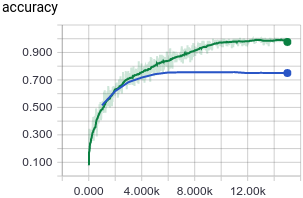
\includegraphics[height=4.0cm]{acc-plain.png}\
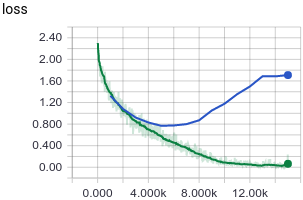
\includegraphics[height=4.0cm]{loss-plain.png}
\caption{Accuracy (left) and loss (right) for the CNN with batch size of $128$ and no regularization. Green lines illustrate performance on the training set and blue lines on the test set.}
\label{fig:1}
\end{figure}
As shown in the Figures~\ref{fig:1}, the model overfits the training data.
The accuracy in the training set approximates $1.0$ in the last $5000$ steps of the training where the loss in the test set is increasing while accuracy in the test set is not affected.


\subsection{Regularization}
\label{sec:reg}

In this section I present the results of the CNN with regularization losses in the weights.
More specifically I added regularization losses in the fully connected layers $fc1, fc2$
\begin{verbatim}
if self.wd is not None:
    weight_decay = tf.mul(tf.nn.l2_loss(w_fc1), self.wd, name='weight_loss')
    tf.add_to_collection('losses', weight_decay)
\end{verbatim}
making sure the losses were added to the loss function in the loss function of convNet class.
Figure~\ref{fig:2} illustrates the accuracy and the loss during training and test with regularization $wd=0.005$.
\begin{figure}[h!]
\centering
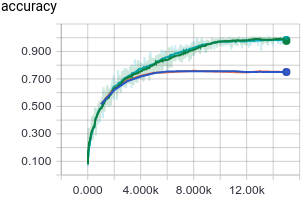
\includegraphics[height=4.0cm]{acc-plain-reg.png}\
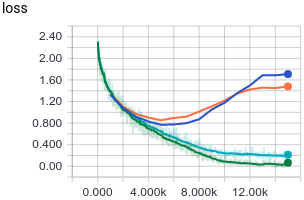
\includegraphics[height=4.0cm]{loss-plain-reg.png}
\caption{Accuracy (left) and loss (right) for the CNN with batch size of $128$ and no regularization. Cyan lines illustrate performance on the training set and orange lines on the test set.}
\label{fig:2}
\end{figure}
There is no performance gain by the regularization apart from a decrease in the loss in the test set.




\subsection{Dropout}

In the next experiment I implemented dropout in the fully connected layers $fc1, fc2$.
\begin{verbatim}
h_fc1 = tf.cond(tf.cast(self.isTrain, tf.bool), 
lambda: tf.nn.dropout(h_fc1, 0.8), lambda: h_fc1)
\end{verbatim}
Figure~\ref{fig:3} illustrates the accuracy and the loss during training and test with dropout $0.5, 0.2$.
\begin{figure}[h!]
\centering
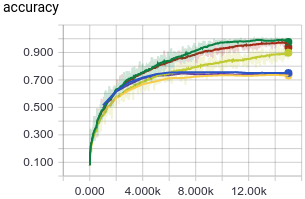
\includegraphics[height=4.0cm]{acc-plain-drop.png}\
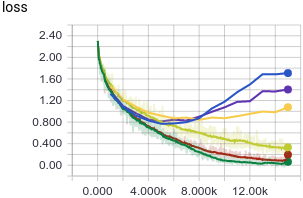
\includegraphics[height=4.0cm]{loss-plain-drop.png}
\caption{Accuracy (left) and loss (right) for the CNN with batch size of $128$ and dropout. Red lines illustrate performance on the training set and purple lines on the test set for dropout $0.2$, while light green lines illustrate performance on the training set and yellow lines on the test set for dropout $0.5$.}
\label{fig:3}
\end{figure}
The performance on the test set in the end of the training was:
\begin{itemize}
\item For no dropout: $\mathbf{0.7503}$
\item For dropout $0.5$: $0.7324$
\item For dropout $0.2$: $0.7433$
\end{itemize}
There was no performance gain, but only a decrease in overfitting with dropout $0.5$.


\subsection{Smaller Batch Size}

Here, I used half the size of the batch to complete training using batch size of $64$.
Figure~\ref{fig:4} illustrates the accuracy and the loss during training and test with the given batch size of $128$ and the half batch size of $64$.

\begin{figure}[h!]
\centering
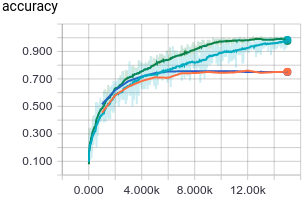
\includegraphics[height=4.0cm]{acc-linear-64.png}\
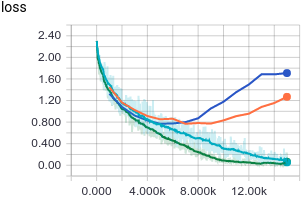
\includegraphics[height=4.0cm]{loss-linear-64.png}
\caption{Accuracy (left) and loss (right) for the CNN with batch size of $64$. Cyan lines illustrate performance on the training set and orange lines on the test set for dropout $0.2$. Green and blue lines illustrate the performance of batch size $128$ with default configuration CNN as in all previous figures.}
\label{fig:4}
\end{figure}
The performance on the test set in the end of the training was:
\begin{itemize}
\item For batch size $128$: $0.7503$
\item For batch size $64$: $\mathbf{0.7520}$
\end{itemize}
There was a performance gain by using smaller batch size and a limited overfitting.

\subsubsection{Regularization}
As in Section~\ref{sec:reg} I used regularization for the weights in the fully connected layers $fc1, fc2$.
Figure~\ref{fig:5} illustrates the accuracy and the loss during training and test with the given batch size of $64$ two regularization values for the weight decays.

\begin{figure}[h!]
\centering
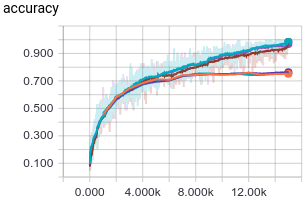
\includegraphics[height=4.0cm]{acc-linear-64-reg.png}\
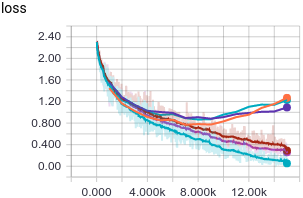
\includegraphics[height=4.0cm]{loss-linear-64-reg.png}
\caption{Accuracy (left) and loss (right) for the CNN with batch size of $64$. Cyan lines illustrate performance on the training set and orange lines on the test set without weight regularization. Red lines illustrate performance on the training set and purple lines on the test set with weight regularization $0.01$. Light purple lines illustrate performance on the training set and cyan lines on the test set with weight regularization $0.005$.}
\label{fig:5}
\end{figure}
The performance on the test set in the end of the training was:
\begin{itemize}
\item No regularization: $0.7520$
\item For regularization $0.01$: $\mathbf{0.7634}$
\item For regularization $0.005$: $0.7569$
\end{itemize}
The maximum reported accuracy on the test set was achieved by using mini batches of $64$ size and regularization values of $0.01$.


\subsubsection{Dropout}


\begin{figure}[h!]
\centering
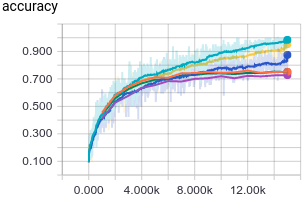
\includegraphics[height=4.0cm]{acc-linear-64-drop.png}\
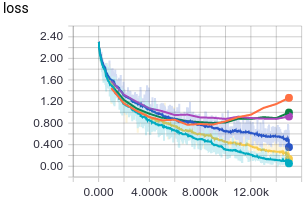
\includegraphics[height=4.0cm]{loss-linear-64-drop.png}
\caption{Accuracy (left) and loss (right) for the CNN with batch size of $64$. Cyan lines illustrate performance on the training set and orange lines on the test set without weight regularization. Red lines illustrate performance on the training set and purple lines on the test set with weight regularization $0.01$. Light purple lines illustrate performance on the training set and cyan lines on the test set with weight regularization $0.005$.}
\label{fig:6}
\end{figure}

The performance on the test set in the end of the training was:
\begin{itemize}
\item No dropout: $0.7520$
\item For dropout $0.5$: $0.7279$
\item For dropout $0.2$: $0.7493$
\end{itemize}
The was no performance gain by using dropout when using smaller batches of $64$ size.


\subsection{Feature Visualization}

In this section I show how the features learned during training of the CNN can be illustrated and how they can be used to train an one-vs-all classifier.
I load the learned weights during training and converting them to $2$-d points using TSNE.
\begin{verbatim}
tsne = TSNE(n_components=2, verbose=1, perplexity=40, n_iter=300)
tsne.fit_transform(features)
\end{verbatim}
Figure~\ref{fig:7} presents the visualization of the features in the two dimensional space. 
You can observe that features obtained in $fc2$ layer can distinguish better features of different classes.
On the contrary when see the flatten features all labels are located close to points of other classes.
\begin{figure}[h!]
\centering
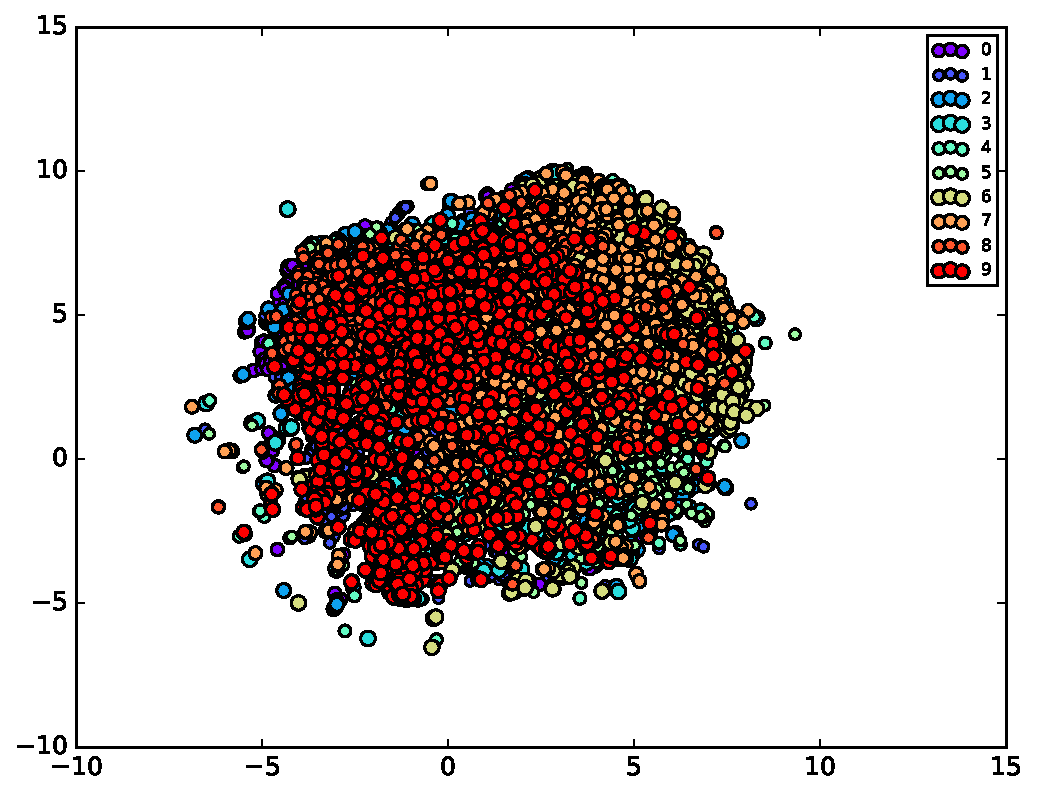
\includegraphics[height=5.0cm]{visualization-linear-features_flatten.pdf}
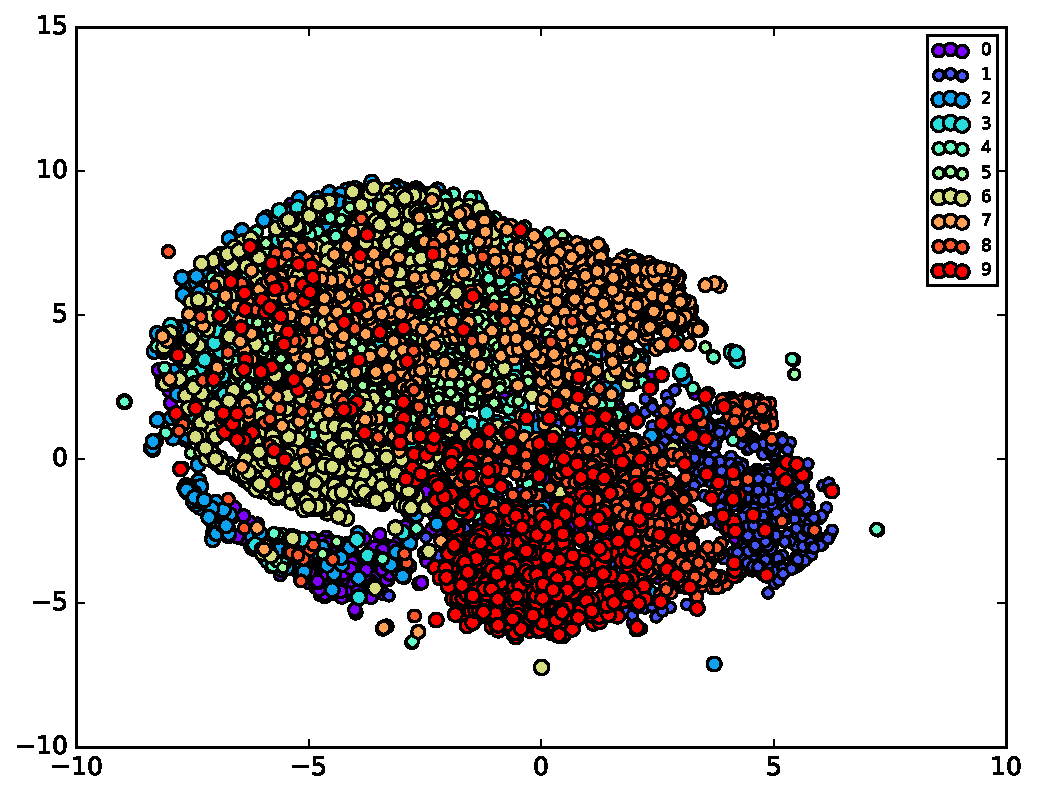
\includegraphics[height=5.0cm]{visualization-linear-features_fc1.pdf}
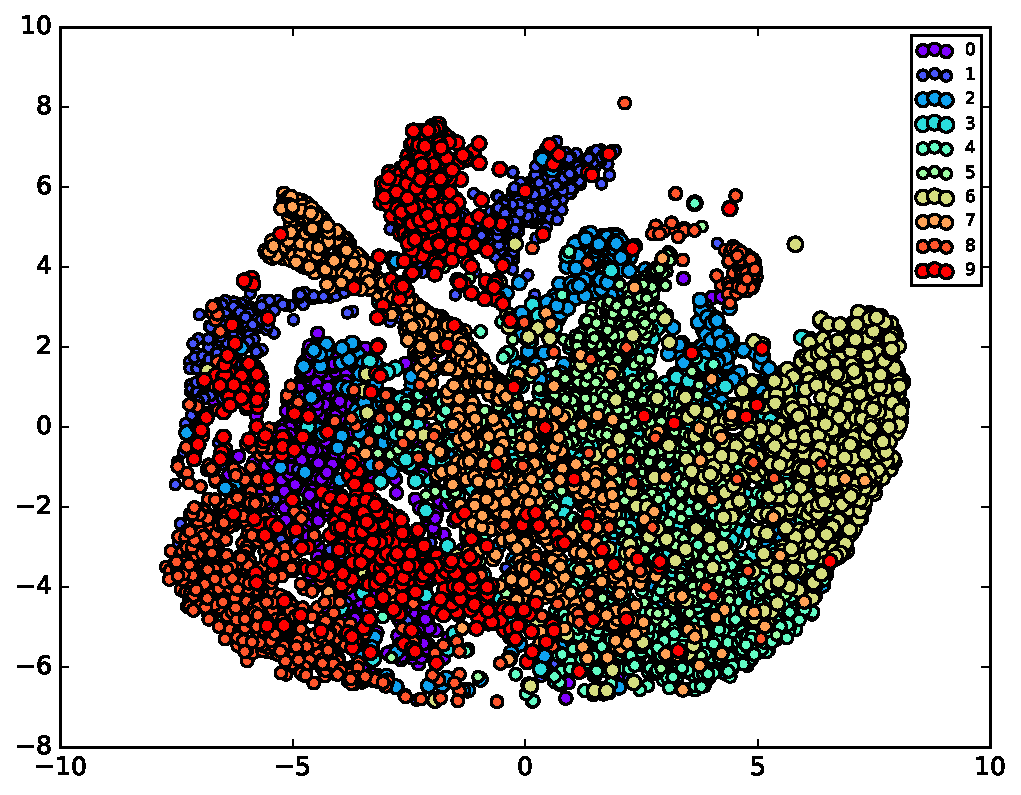
\includegraphics[height=5.0cm]{visualization-linear-features_fc2.pdf}
\caption{Visualization of the features in the 2-d space of the \texttt{flatten} layer (top), \texttt{fc1} (bottom-left), \texttt{fc2} (bottom-right).}
\label{fig:7}
\end{figure}

\subsubsection{One-vs-Rest Classifier}


To test the accuracy of the one-vs-all classifier I use the features retained by the learned model to train the classifiers.
Using the 80 percent of the features I train a linear kernel OneVsRest classifier, and test the accuracy over the rest 20 percent.
\begin{verbatim}
train_set = range(int(features.shape[0]*0.8))
test_set = range(train_set[-1] + 1, features.shape[0])

classif = OneVsRestClassifier(SVC(kernel='linear'))
classif.fit(features[train_set], batch_y[train_set]
classif.score(features[test_set], batch_y[test_set]
\end{verbatim}
Here, the reported accuracy of the one-vs-classifiers on the test set:
\begin{itemize}
\item Accuracy with flatten features: $0.6306$.
\item Accuracy with fc1 features: $0.$.
\item Accuracy with fc2 features: $0.$.
\end{itemize}
It is natural that the accuracy is higher for later layers.
As it was earlier $fc2$ layer can distinguish better features of different classes.




\section{Task 2}

In this section I present my implementation and the results achieved by the siamese architecture of the CNN.
First, I implemented the functions \texttt{create\_dataset} and \texttt{next\_batch} in the \texttt{cifar10\_siamese\_utils.py}.


\subsection{Dataset}

The create\_dataset function:
\begin{tiny}
\begin{verbatim}
dset = []
    for sample_tuple in range(num_tuples):

        n_correct = int(fraction_same * batch_size)

        val_set_indexes = range(int(source_data.train._images.shape[0] * 0.8), source_data.train._images.shape[0])

        index_x1 = np.random.choice(val_set_indexes)
        label_x1 = source_data.train._labels[index_x1]

        index_x2_similar = np.random.choice(val_set_indexes[0] +
                                            np.where(source_data.train._labels[val_set_indexes] == label_x1)[0],
                                            replace=False, size=n_correct)

        index_x2_opposite = np.random.choice(val_set_indexes[0] +
                                             np.where(source_data.train._labels[val_set_indexes] != label_x1)[0],
                                             replace=False, size=(batch_size - n_correct))

        x1 = np.array([source_data.train._images[index_x1] for i in range(batch_size)])
        x2 = source_data.train._images[index_x2_similar]
        x2 = np.vstack((x2, source_data.train._images[index_x2_opposite]))
        labels = np.hstack((np.ones((n_correct)), np.zeros((batch_size - n_correct))))

        dset.append((x1, x2, labels))

    return dset
\end{verbatim}
\end{tiny}
which returns \texttt{num\_tuples} tuples of the following batches:
\begin{verbatim}
      X_1            X_2               Y
| image_cl1_1, image_cl1_10  | -->   | 1 |
| image_cl1_1, image_cl1_4   | -->   | 1 |
| image_cl1_1, image_cl1_163 | -->   | 1 |
| image_cl1_1, image_cl1_145 | -->   | 1 |
| image_cl1_1, image_cl3_8   | -->   | 0 |
|      .            .        | -->   | 0 |
|      .            .        | -->   | 0 |
|      .            .        | -->   | 0 |
| image_cl1_1, image_cl5_8   | -->   | 0 |
| image_cl1_1, image_cl2_    | -->   | 0 |
| image_cl1_1, image_cl10_8  | -->   | 0 |
\end{verbatim}
and used for the evaluation of the training set.


The \texttt{next\_batch} function, which include the following piece of code was given to us in \texttt{cifar10\_utils.py} to sample as uniformly the dataset as possible.
\begin{tiny}
\begin{verbatim}
n_correct = int(fraction_same * batch_size)
        val_set_indexes = range(int(self._images.shape[0] * 0.8))

        start = self._index_in_epoch
        self._index_in_epoch += batch_size
        if self._index_in_epoch > self._num_examples * 0.8:
            self._epochs_completed += 1
            np.random.shuffle(val_set_indexes)
            start = 0
            self._index_in_epoch = batch_size
            assert batch_size <= self._num_examples

        end = self._index_in_epoch

        val_set_indexes = val_set_indexes[start:end]
\end{tiny}
\end{verbatim}
\end{tiny}
The \texttt{next\_batch} function then creates each training batch in two following ways.
\begin{itemize}
\item In the \emph{default} implementation the structure of each batch is the same as the test set following the same idea.
All images in $x1$ are the same, while $x2$ contains \texttt{fraction} percentage of similar label images to $x1$ and the rest random images of different classes.
\item In the \emph{alternative} implementation the following piece of code
\begin{tiny}
\begin{verbatim}
random_index = np.array(np.random.choice(val_set_indexes, replace=False, size=batch_size))

matches = [np.random.choice(np.array(np.where(self._labels[range(int(self._images.shape[0] * 0.8))] == 
self._labels[x]))[0]) for x in random_index]

mismatches = [np.random.choice(np.array(np.where(self._labels[range(int(self._images.shape[0] * 0.8))] != 
self._labels[x]))[0]) for x in random_index]

x1 = self._images[random_index]
x2 = self._images[matches[:n_correct]]
x2 = np.vstack((x2, self._images[mismatches[n_correct:]]))
labels = np.hstack((np.ones((n_correct)), np.zeros((batch_size-n_correct))))
\end{verbatim}
\end{tiny}
generates batches of random pairs of images respecting the \texttt{fraction} of same label images.
The resulted batch 
\begin{verbatim}
      X_1            X_2               Y
| image_cl1_10, image_cl1_50   | -->   | 1 |
| image_cl4_17, image_cl4_234  | -->   | 1 |
| image_cl8_654, image_cl8_14  | -->   | 1 |
| image_cl8_66, image_cl6_234  | -->   | 0 |
|      .            .          | -->   | 0 |
|      .            .          | -->   | 0 |
|      .            .          | -->   | 0 |
| image_cl2_327, image_cl6_234 | -->   | 0 |
\end{verbatim}
\end{itemize}


\subsection{Loss function}

I used the following two loss functions:
\begin{enumerate}
\item $\mathcal{L} =  Y * \frac{1}{2} * d^2 + (1-Y) * max(margin - d^2, 0)$
\item $\mathcal{L} =  Y * d^2 + (1-Y) * max(margin - d^2, 0)$
\end{enumerate}


\subsection{Training}

\begin{figure}[h!]
\centering
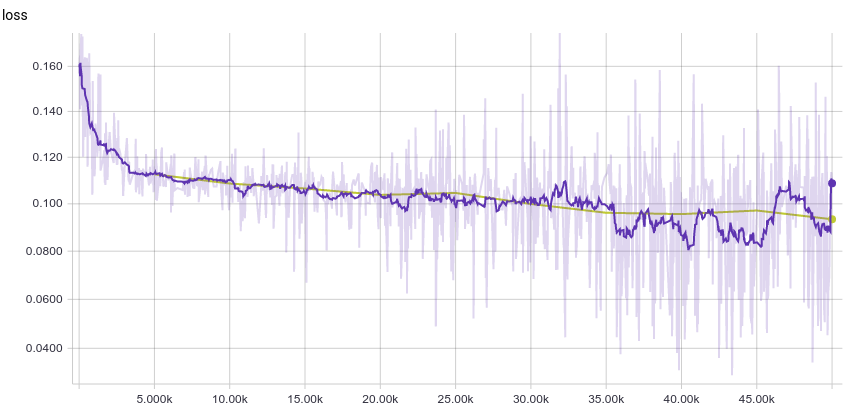
\includegraphics[width=10.2cm]{siamese.png}
\caption{\textbf{Experiment 1} Loss in the training (purple line) and the test set (yellow line) for $50000$ training steps, $margin = 1.0$, using the default \texttt{next\_batch} method and the loss function (1).}
\label{fig:siamese}
\end{figure}



\begin{figure}[h!]
\centering
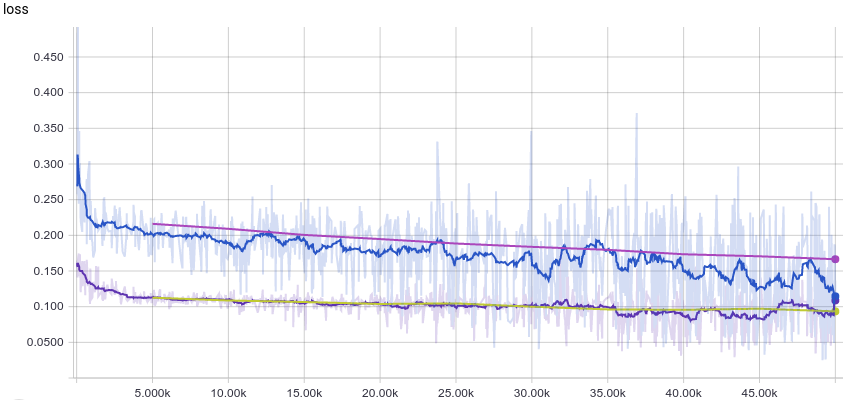
\includegraphics[width=10.2cm]{siamese-1.png}
\caption{\textbf{Experiment 2} Loss in the training (blue line) and the test set (light purple line) for $50000$ training steps, $margin = 1.0$, using the default \texttt{next\_batch} method and the loss function (2).
Loss in the training (purple line) and the test set (yellow line) for $50000$ training steps, $margin = 1.0$, using the default \texttt{next\_batch} method and the loss function (1).}
\label{fig:siamese-1}
\end{figure}


\begin{figure}[h!]
\centering
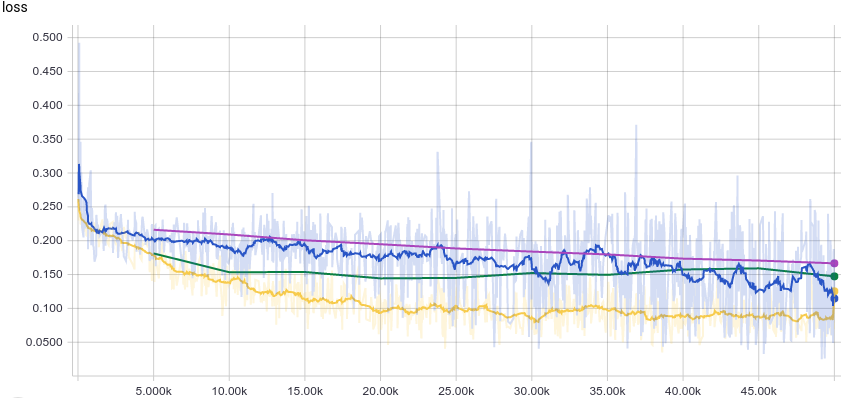
\includegraphics[width=10.2cm]{siamese-2.png}
\caption{\textbf{Experiment 3} Loss in the training (blue line) and the test set (light purple line) for $50000$ training steps, $margin = 1.0$, using the default \texttt{next\_batch} method and the loss function (2).
Loss in the training (yellow line) and the test set (light purple line) for $50000$ training steps, $margin = 1.0$, using the default \texttt{next\_batch} method and the loss function (2).}
\label{fig:siamese-2}
\end{figure}




\subsection{Feature Visualization}

\begin{figure}[h!]
\centering
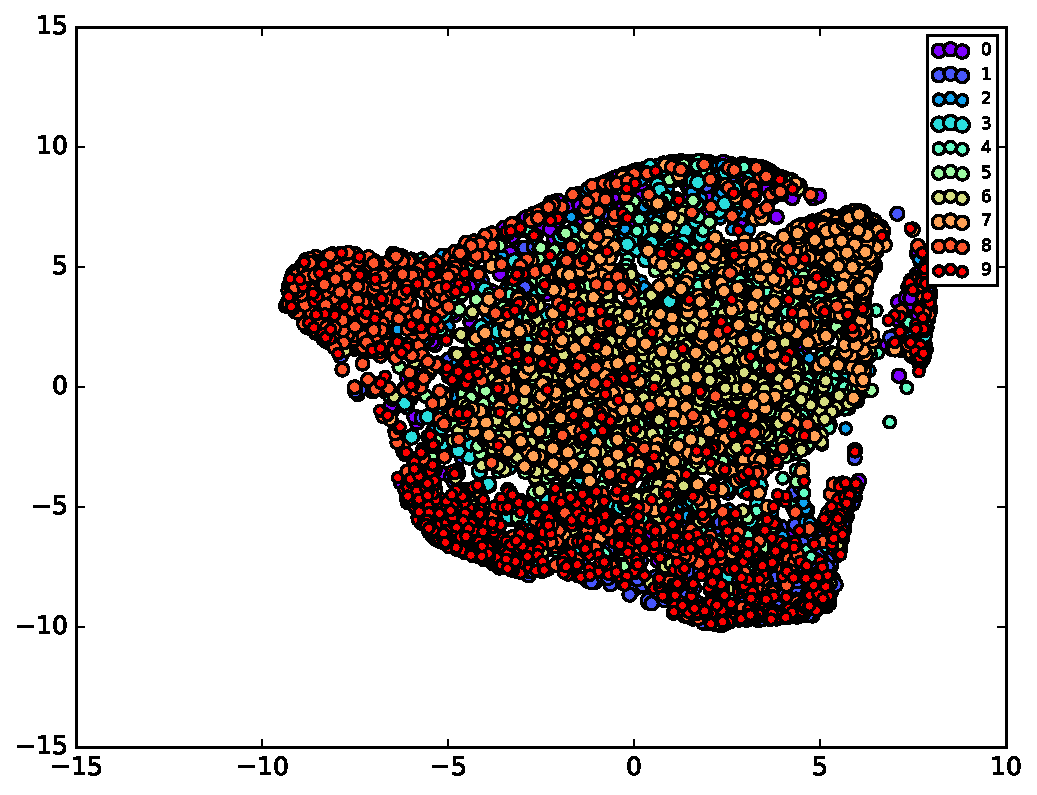
\includegraphics[width=6.2cm]{visualization-siamese-plain.pdf}
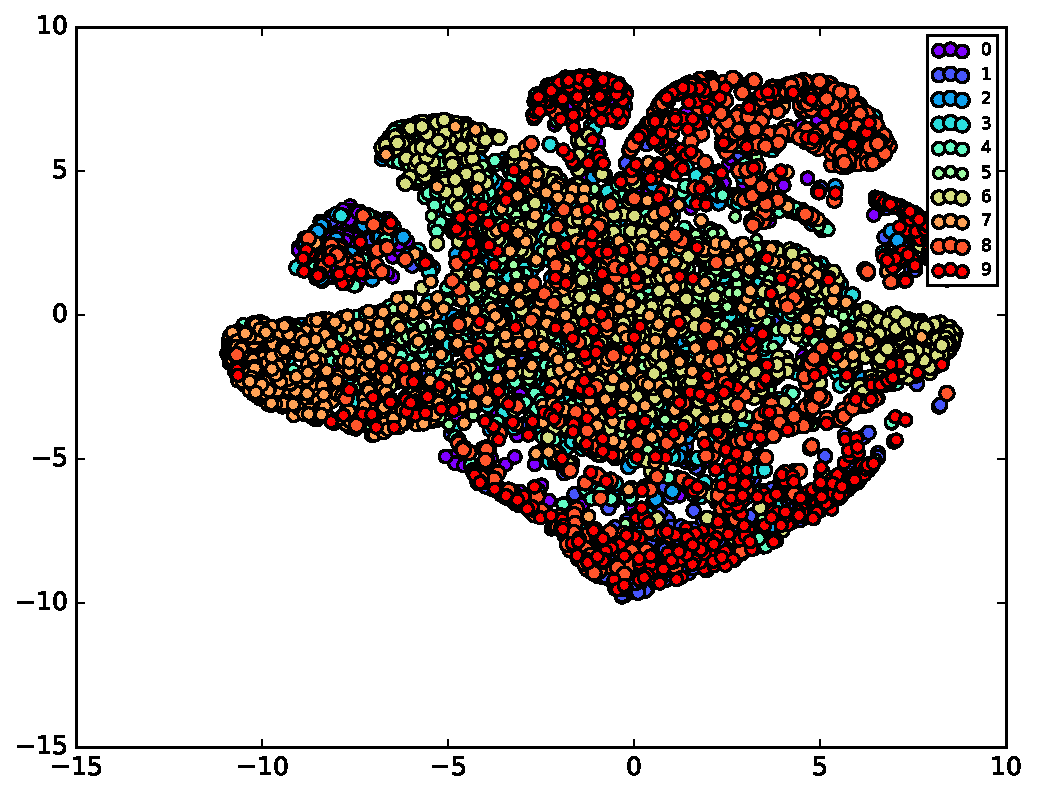
\includegraphics[width=6.2cm]{visualization-siamese-1.pdf}
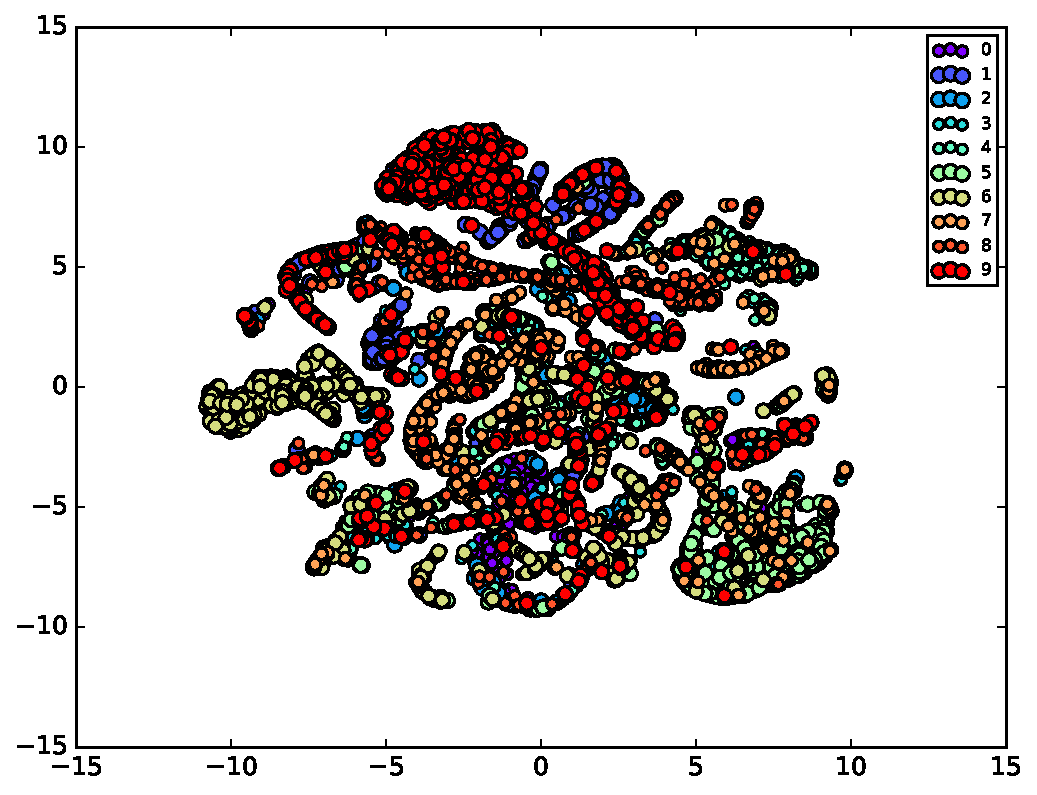
\includegraphics[width=7.2cm]{visualization-siamese-3.pdf}
\caption{}
\label{fig:features}
\end{figure}


\subsection{One-vs-Rest Classifier}
Here, I present the accuracy of the one-vs-rest classifier on the features learned from in the final layer of the siamese network for all experiments
\begin{itemize}
\item \textbf{Experiment 1}: $0.476$
\item \textbf{Experiment 2}: $0.473$
\item \textbf{Experiment 3}: $\mathbf{0.682}$
\end{itemize}

\section{Transfer Learning}
 
 
 \begin{figure}[h!]
\centering
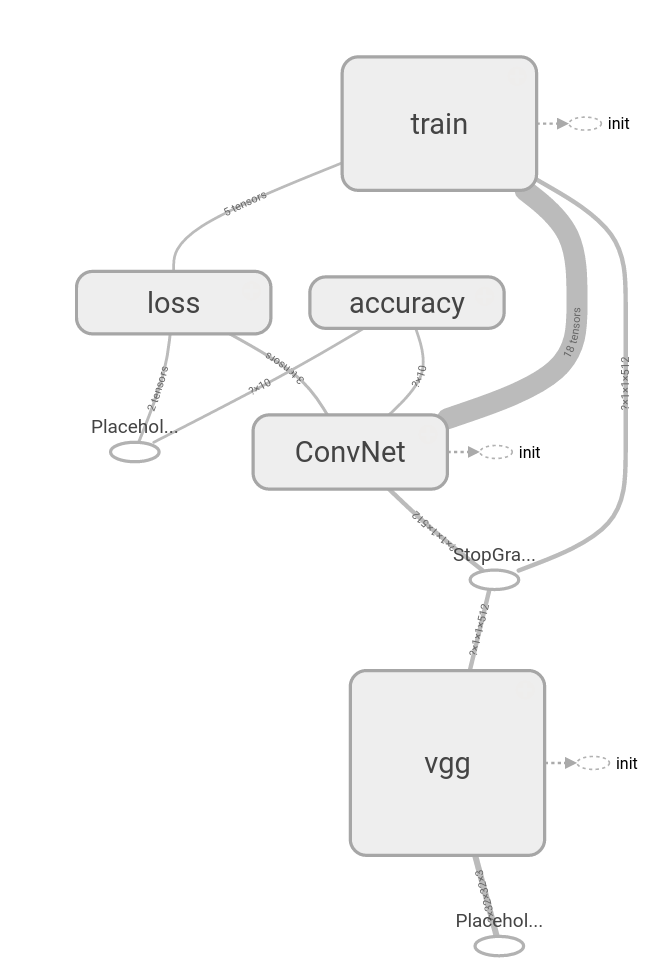
\includegraphics[width=5.2cm]{graph.png}
\caption{Graph for the task 3 of the assignment, the final three layers of convnet were used. Note the stop gradient operation, where we don't want to update the pre-trained weights.}
\label{fig:features}
\end{figure}
 
%
%Using the same TSNE algorithm we present the $2$-dimensional representation of the feat
%\section{Conclusion}
%
%In this assignment I implemented a CNN and reported its performance over the CIFAR10 dataset using different parameters.
%I also implemented the siamese architecture which uses two versions of the same CNN to perform learning in order to distinguish between classes.
%The amount of training steps requires for the siamese are higher than the single CNN architecture.
%The time required for the experiments did not let me try more parameter values, therefore I cannot draw any important conclusions regarding the right parameters that should be used for the two different approaches.


\end{document}
